% !TEX encoding = UTF-8 Unicode

\documentclass{standalone}

% packages
\usepackage{float}
\usepackage{tabu}
\usepackage{booktabs}
\usepackage{graphicx}
\usepackage{caption}
\usepackage[export]{adjustbox}
\usepackage[utf8]{inputenc}
%\usepackage[active,pdftex,tightpage]{preview}
\usepackage{newtxtext,newtxmath}

\begin{document}

%\sf
\scriptsize
\centering 

\begin{tabular}{m{0.5\textwidth} m{0.5\textwidth}}
%
\multicolumn{1}{c}{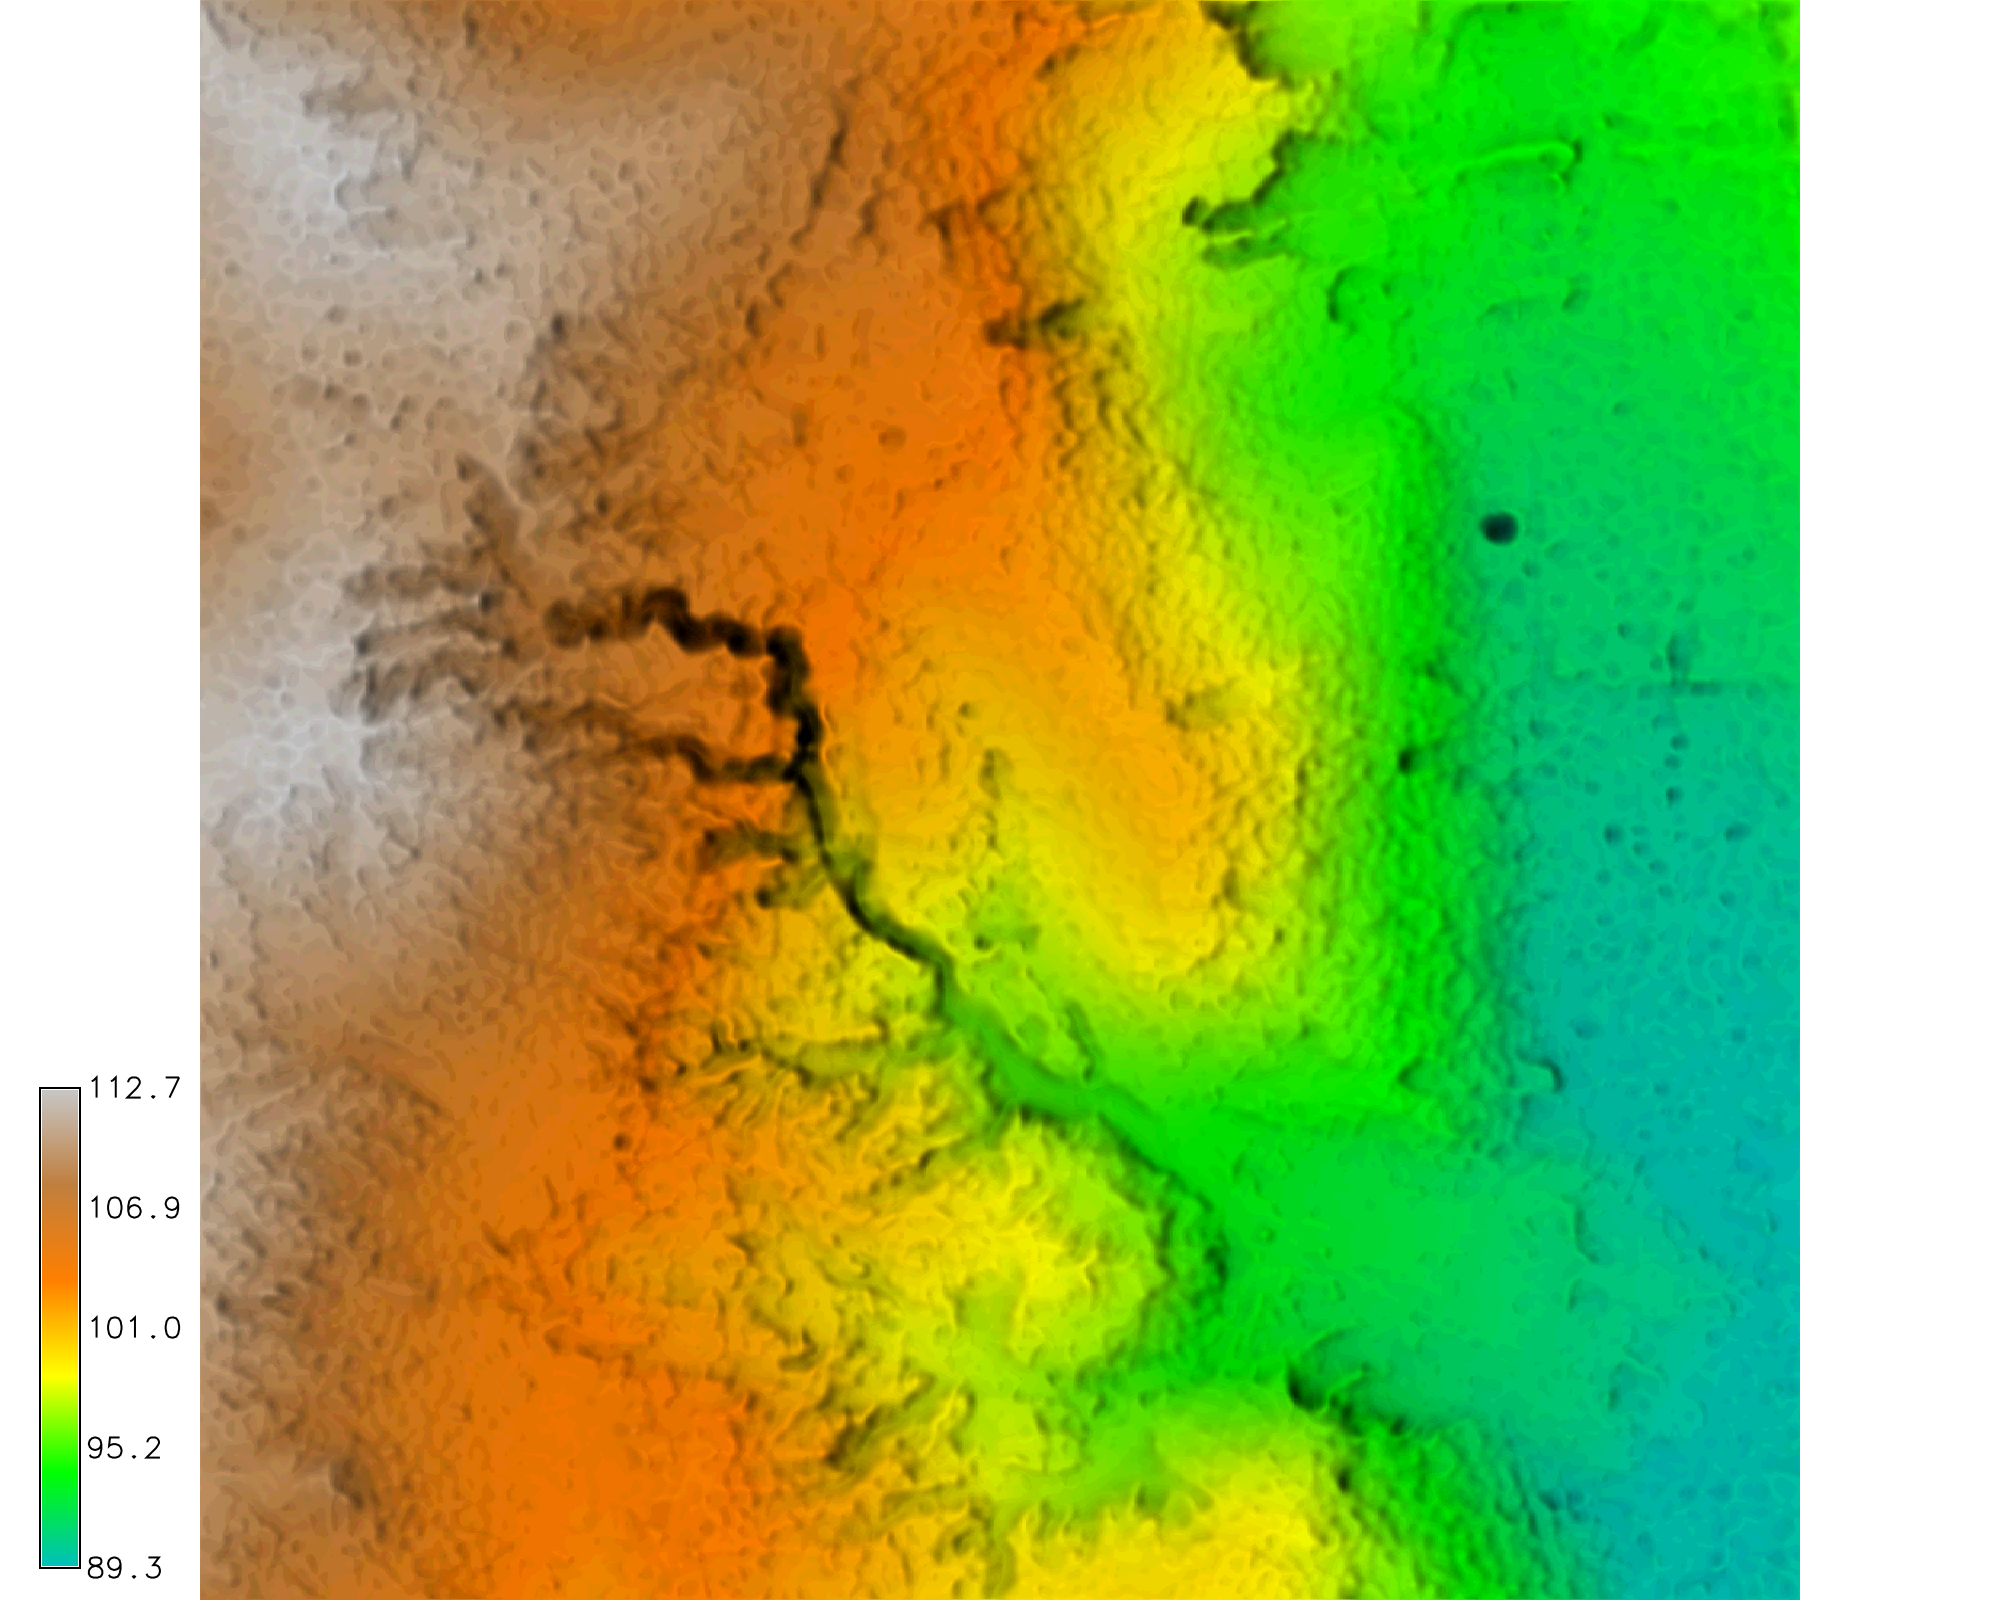
\includegraphics[height=50mm]{../../images/sample_data/elevation_2012.png}} &
\multicolumn{1}{c}{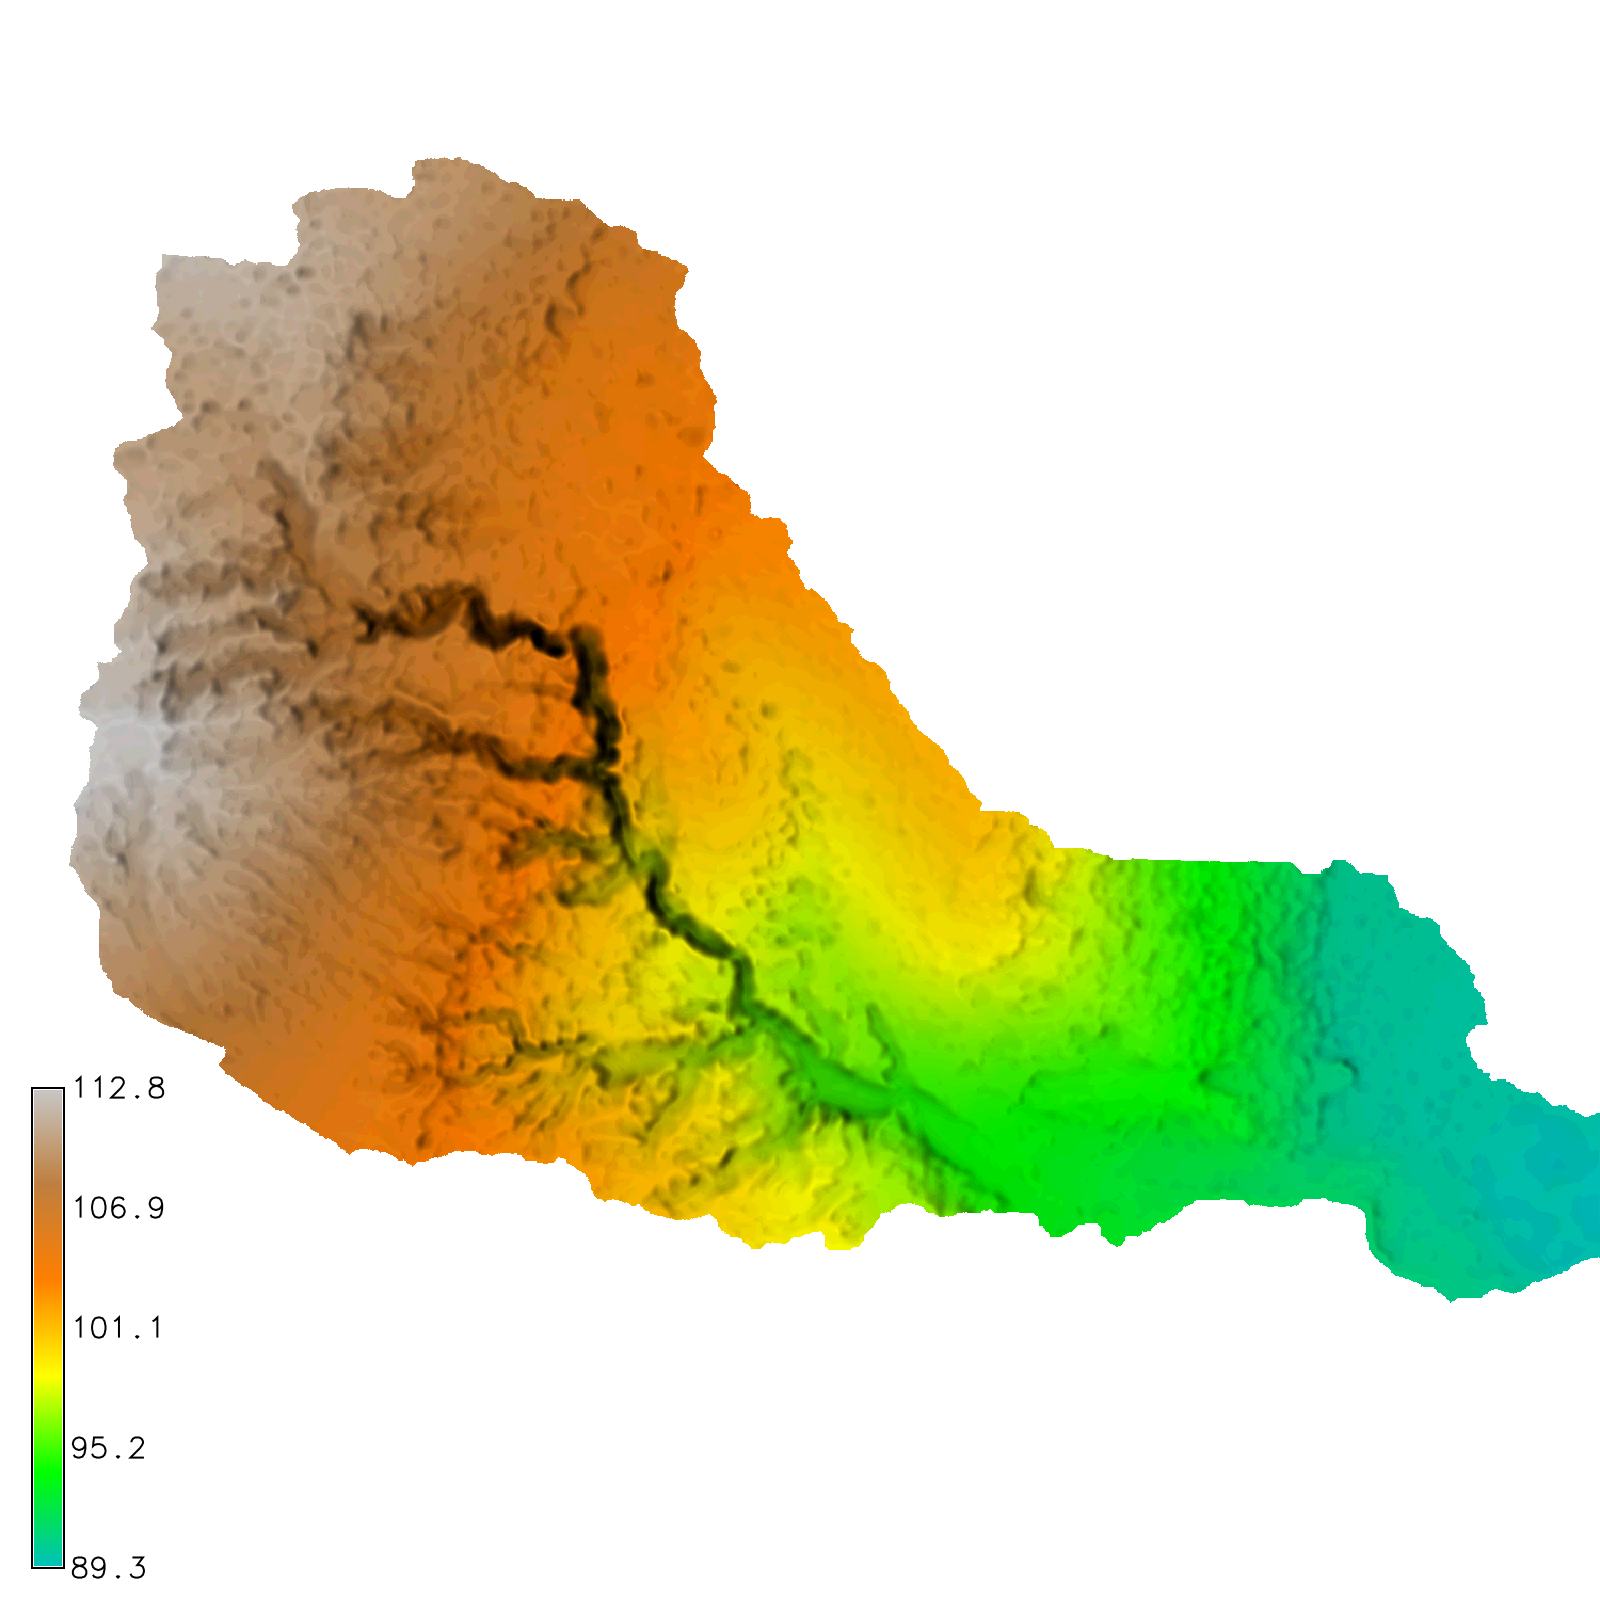
\includegraphics[height=50mm]{../../images/sample_data/elevation_2016.png}}\\
\multicolumn{1}{c}{a. Elevation 2012 $(m)$} & \multicolumn{1}{c}{b. Elevation 2016 $(m)$}\\
%
\multicolumn{1}{c}{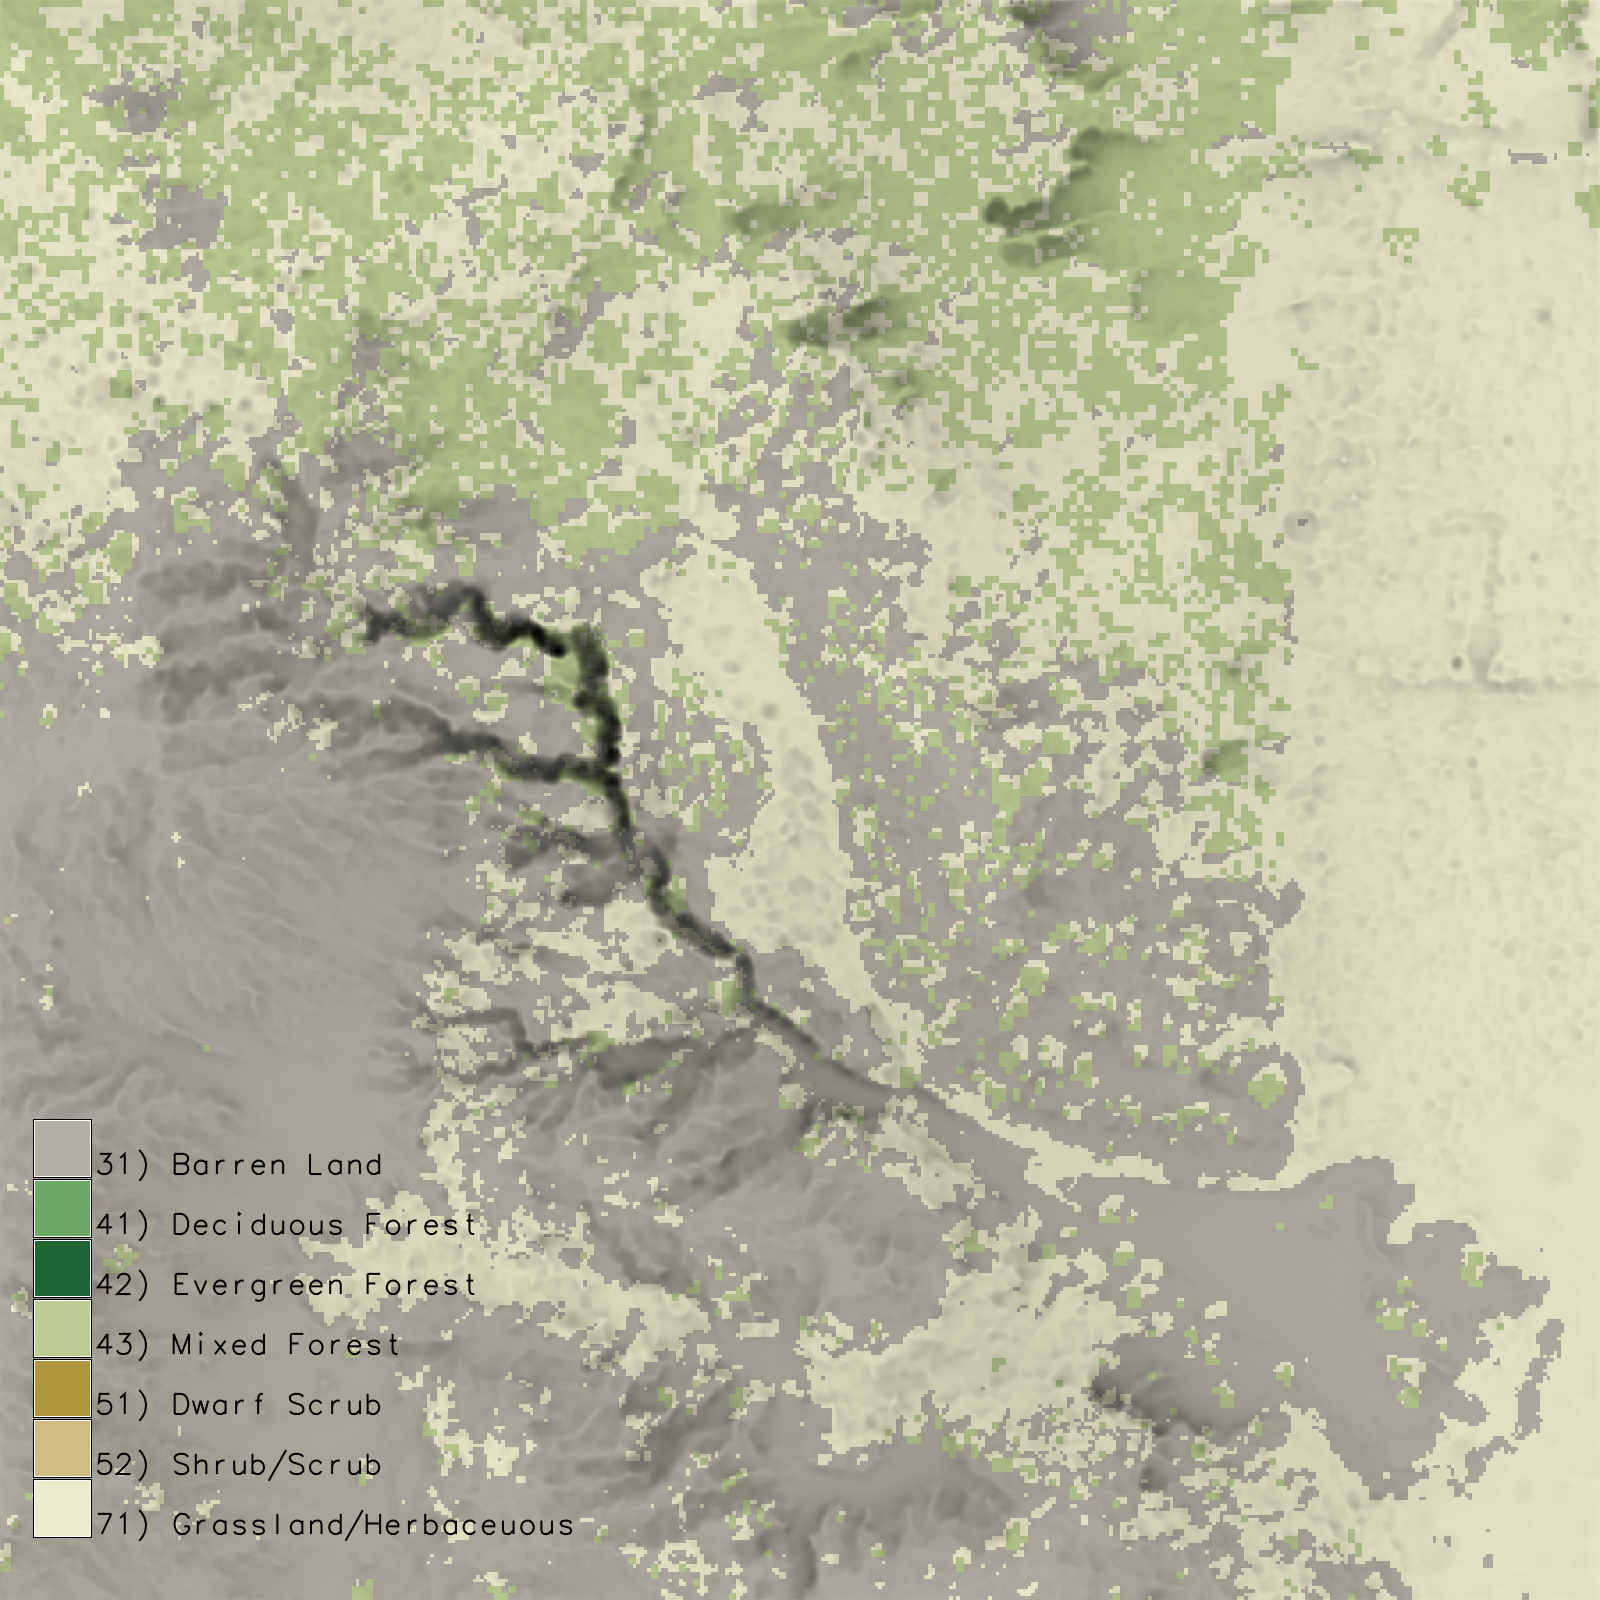
\includegraphics[height=50mm]{../../images/sample_data/landcover.png}} &
\multicolumn{1}{c}{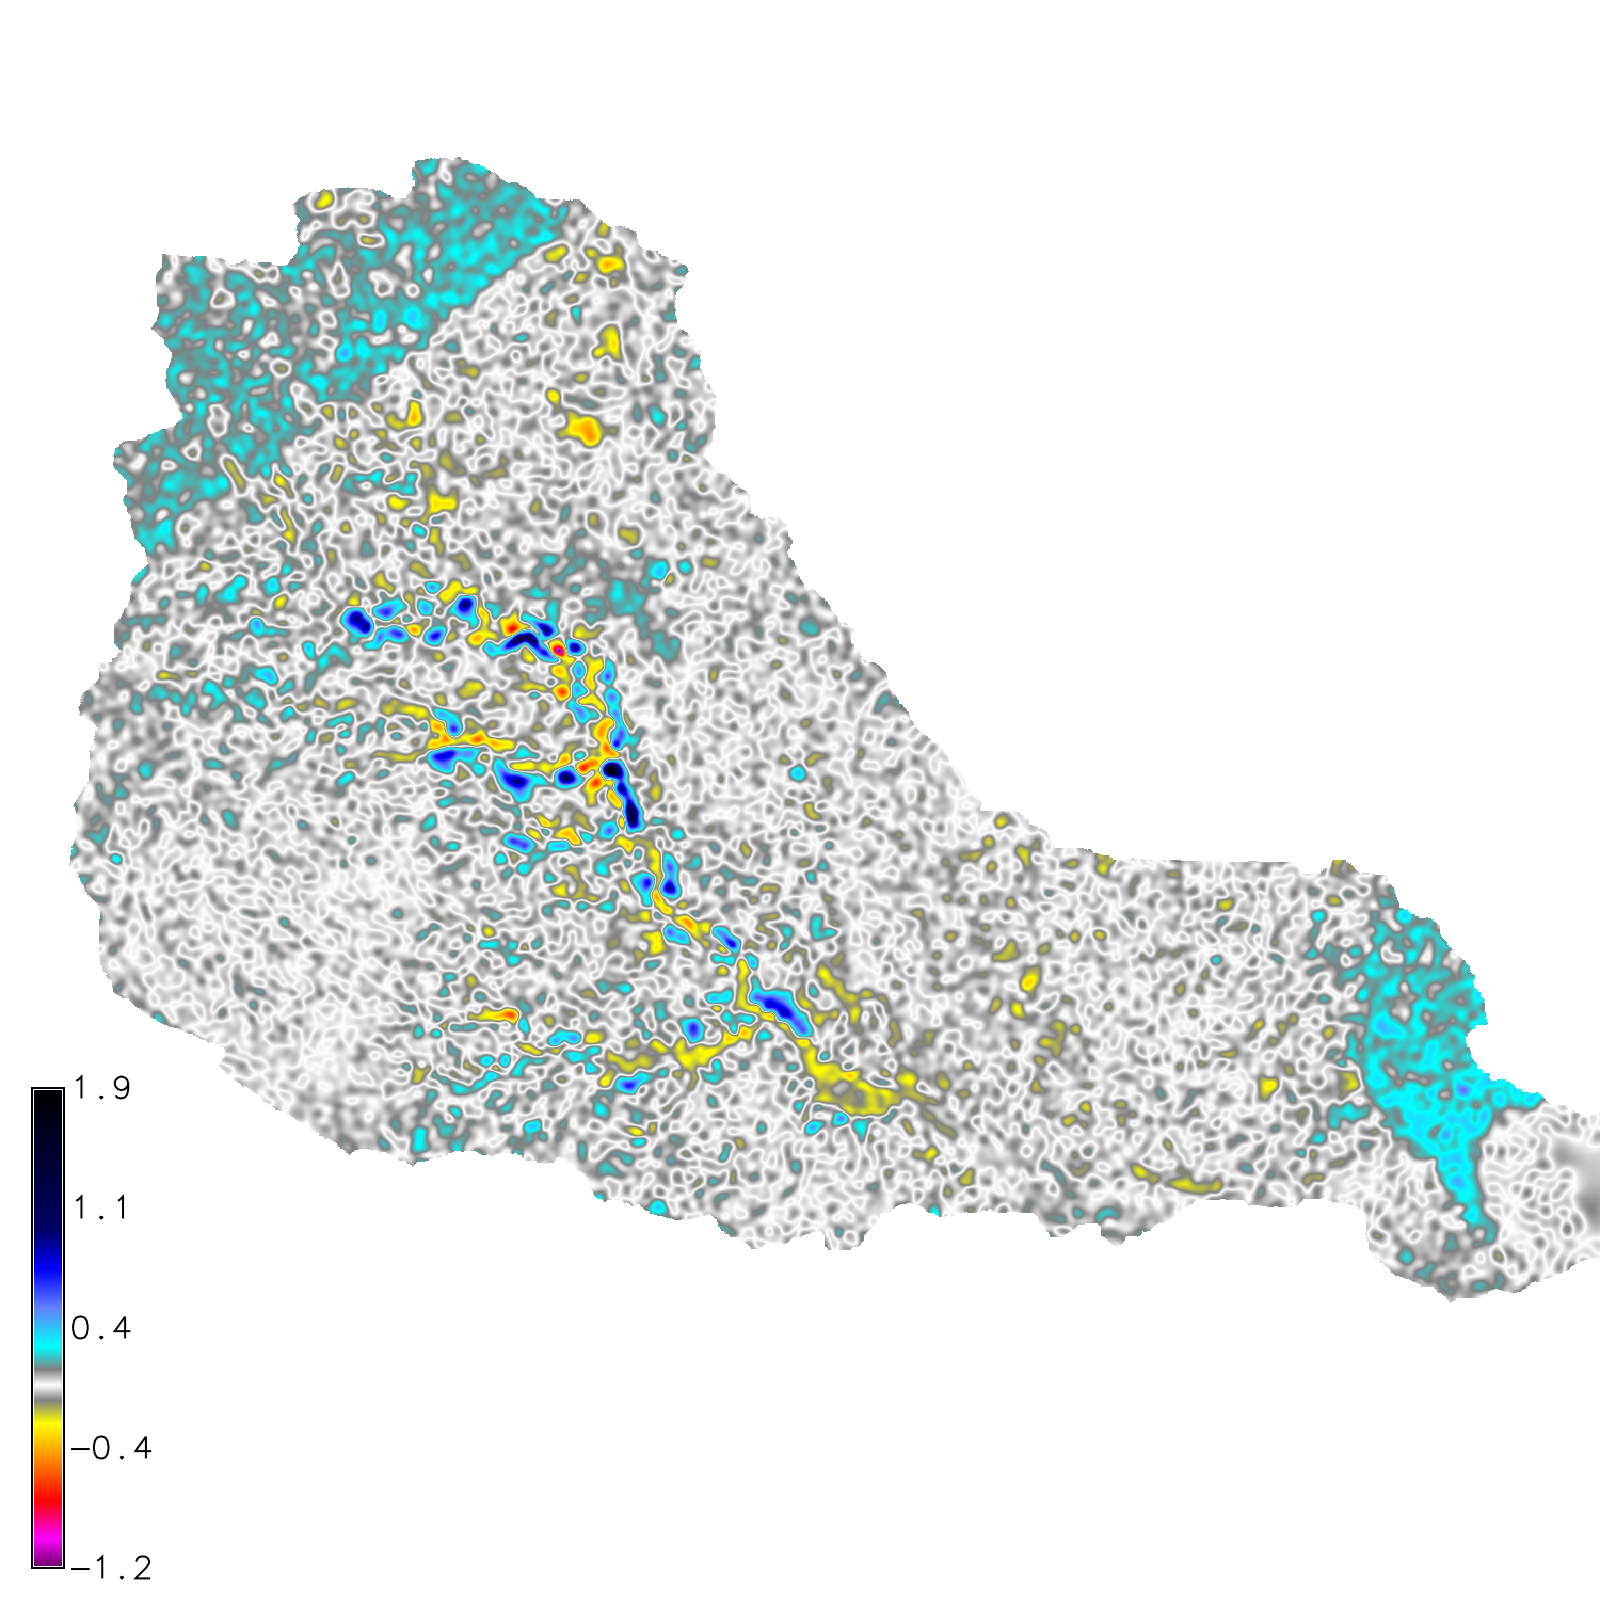
\includegraphics[height=50mm]{../../images/sample_data/difference_2012_2016.png}}\\
\multicolumn{1}{c}{c. Landcover in 2014} & \multicolumn{1}{c}{d. Elevation difference between 2012-2016 $(m)$}\\
%
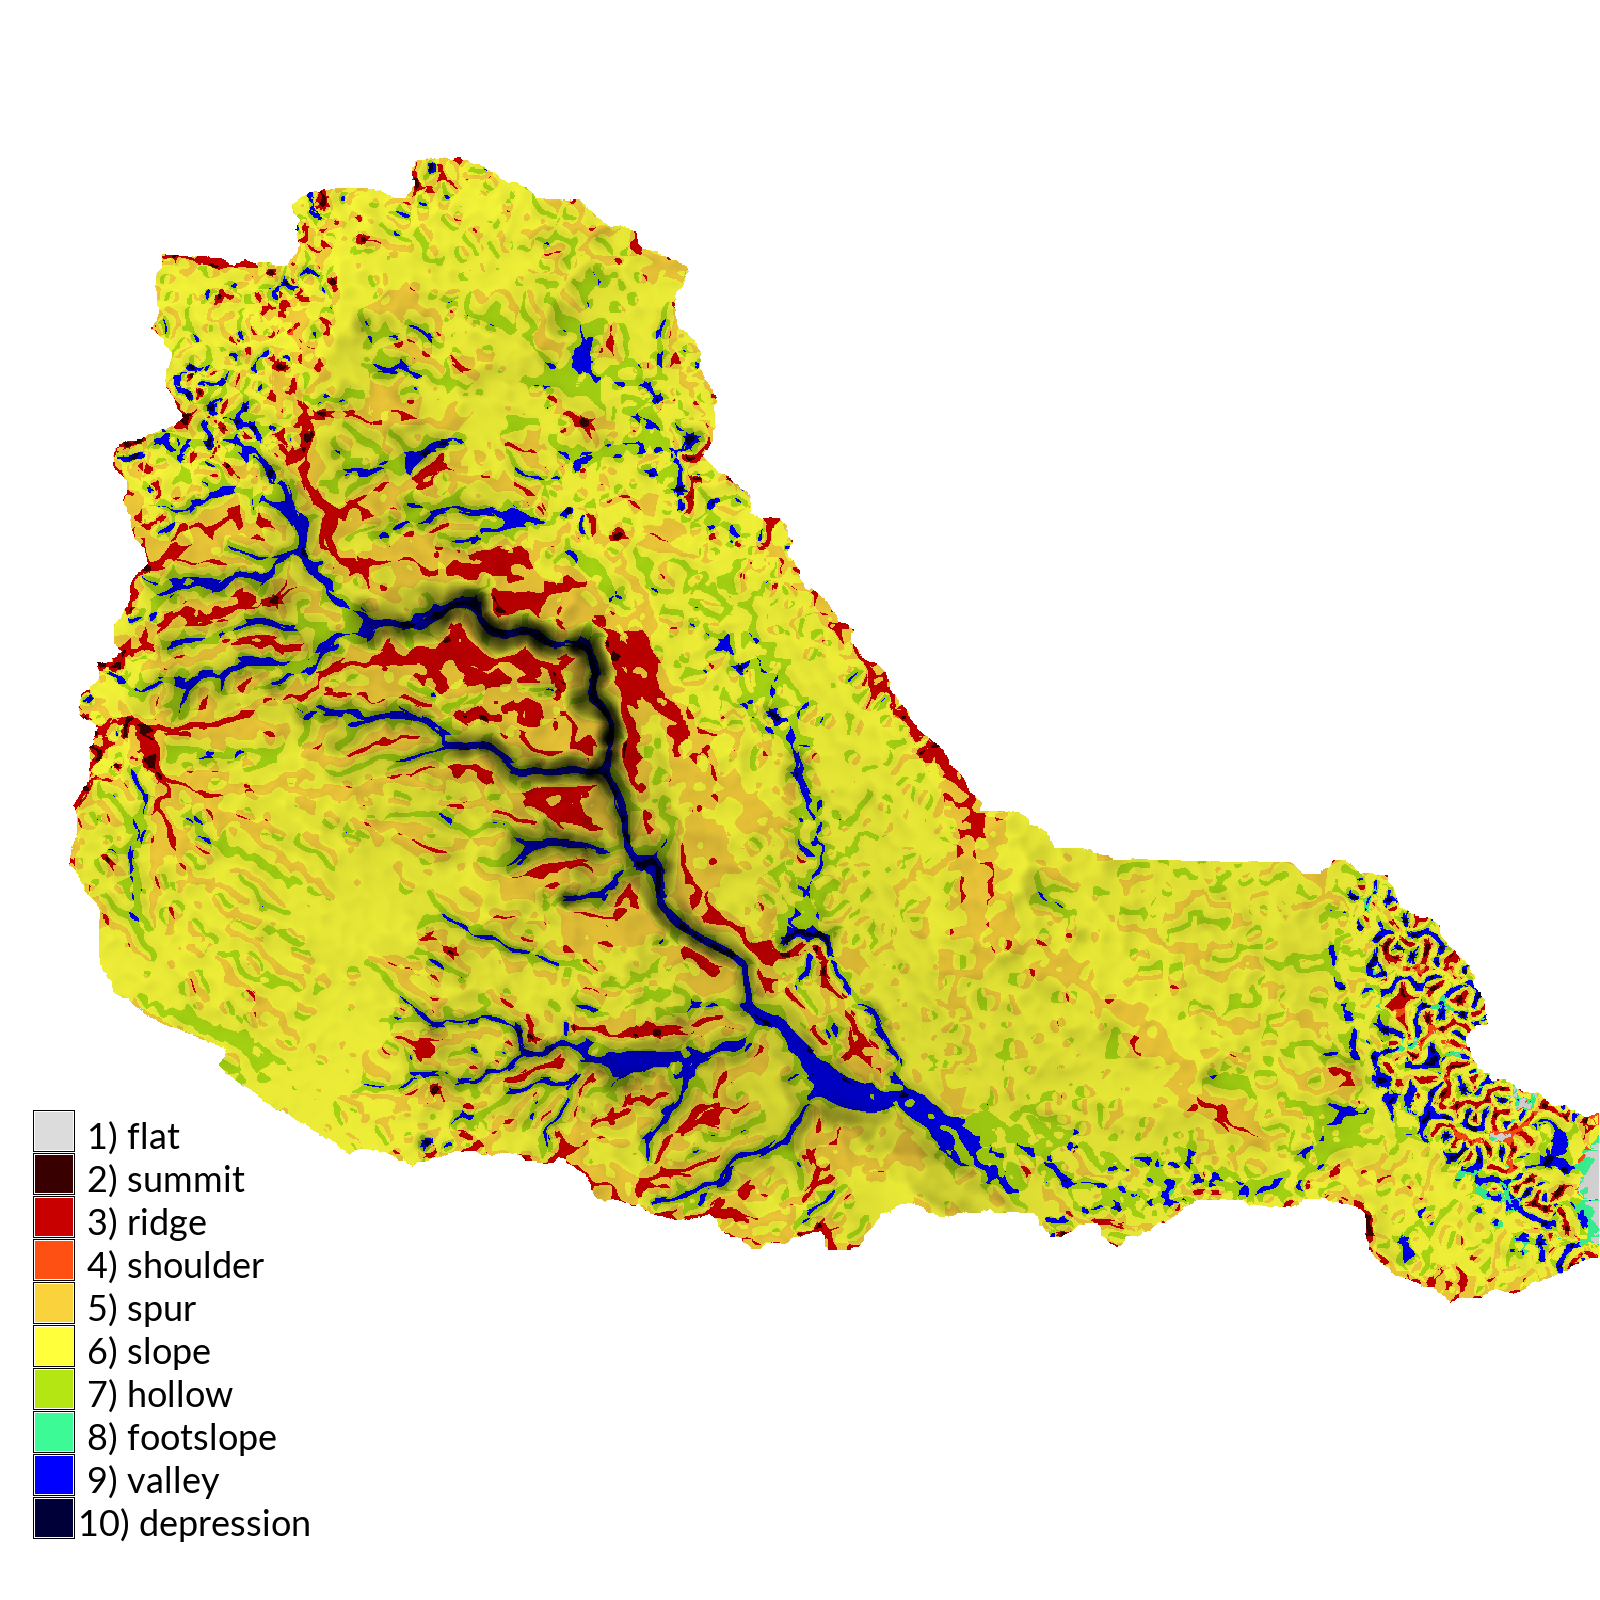
\includegraphics[height=50mm,center]{../../images/sample_data/landforms_2012.png} &
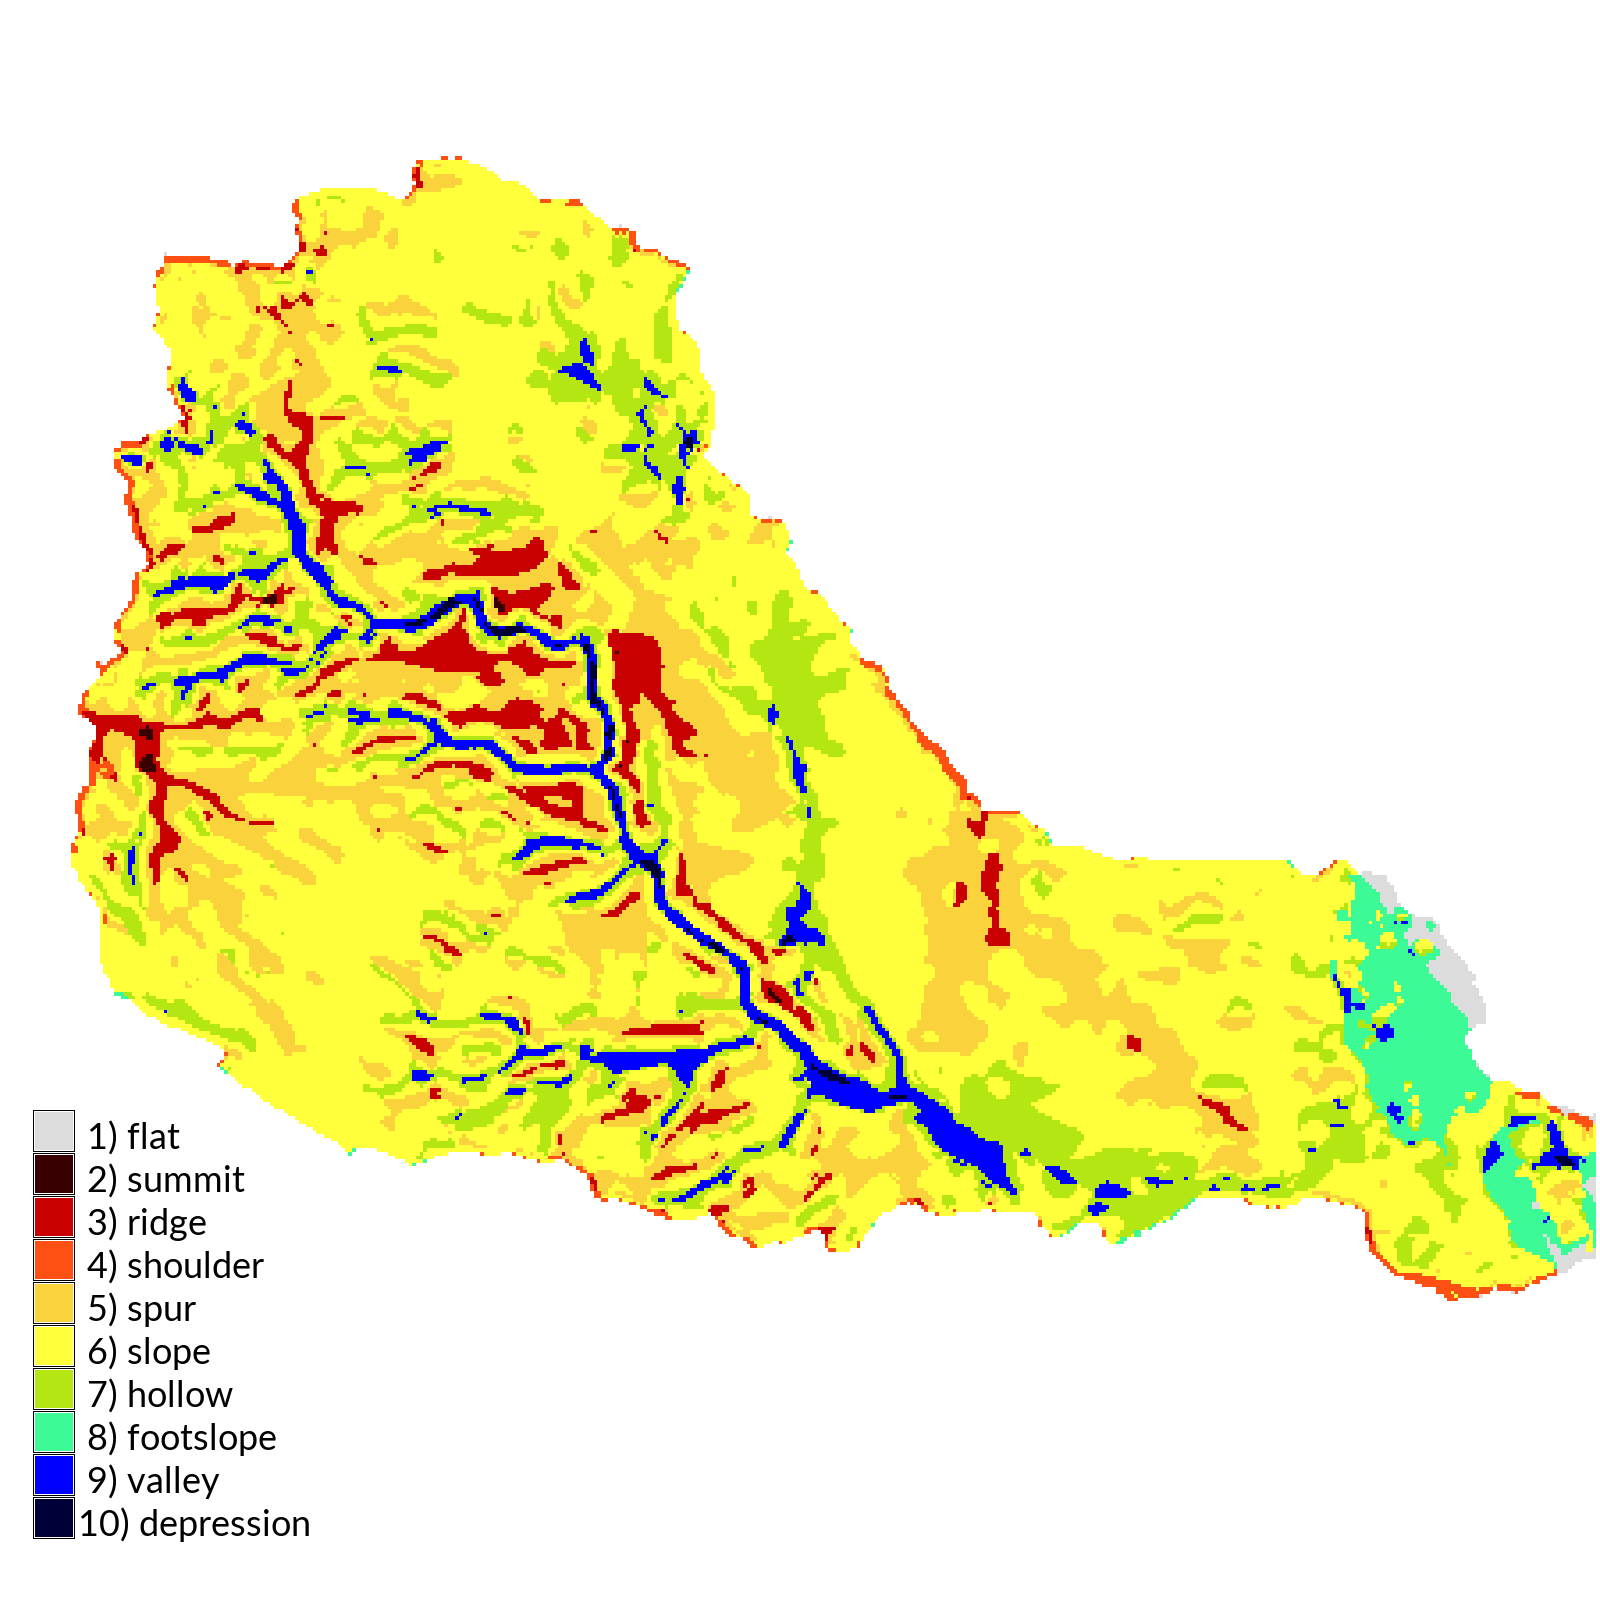
\includegraphics[height=50mm,center]{../../images/sample_data/landforms_2016.png}\\
\multicolumn{1}{c}{e. Landforms 2012} & \multicolumn{1}{c}{f. Landforms 2016}\\
%
\end{tabular}

\end{document}